with steps per year: 7*3600*360
Running velocity verlet
Perihelion position after 100 years: 0.307498, -0.000933806
Perihelion angle after 100 years: -626.38 arc seconds
CPU time: 3248.07


Result:		
	- Find out which initial velocity that gives a circular motion (plot)
\begin{figure}[H]
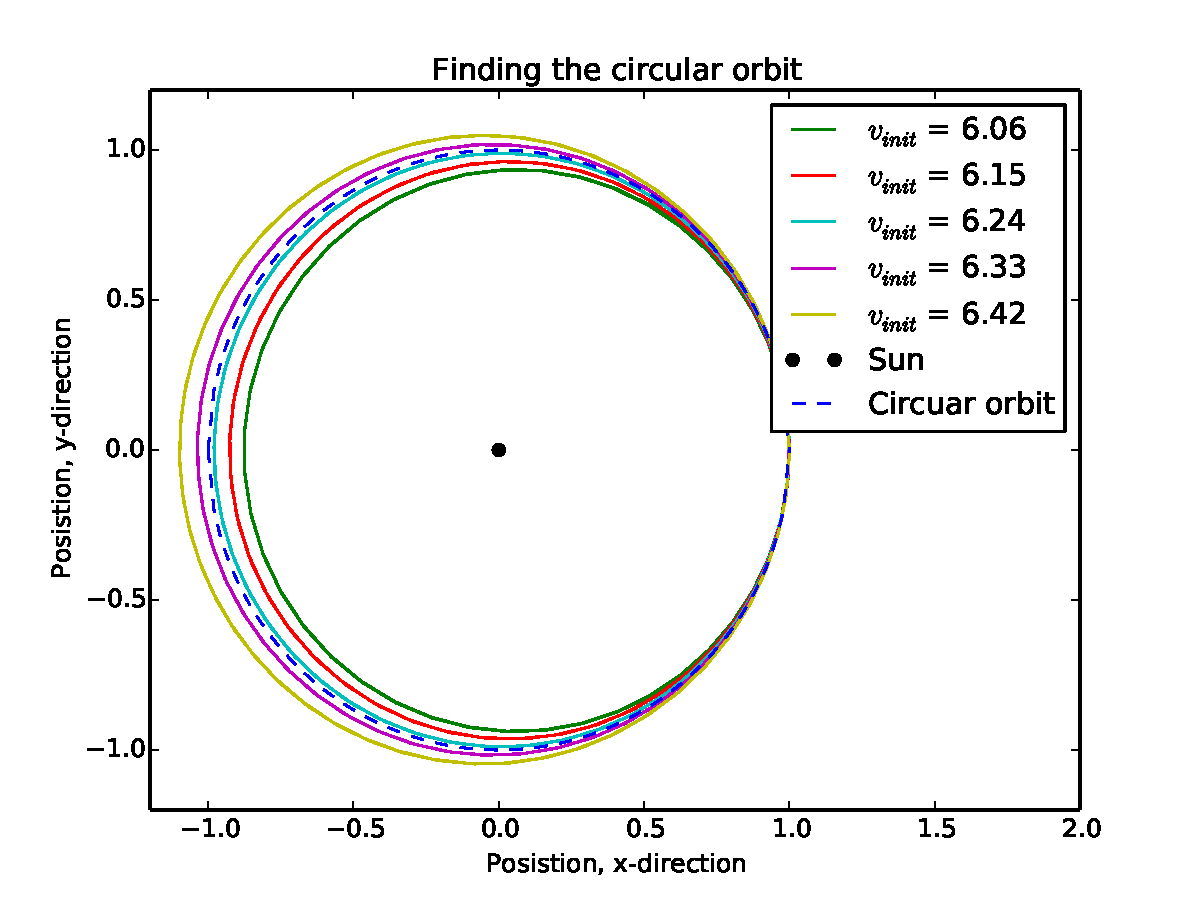
\includegraphics[width=1.1\linewidth]{../results/plots/circular_orbit.pdf}\caption{This is a plt of the orbit with different initial velocities. The circular orbit has a velocity between 6.24 and 6.33. $2 \pi \approx 6.28$ and that is the initial velocity that gives a circular orbit. }\label{fig:circular_orbit}
\end{figure}

	- Test stability (energy-stability) as function of dt (both Verlet and Euler)

Weird results - I think we should look at this tomorrow...	
	
	- Plot the earth orbiting the sun
3 YEARS:
Running velocity verlet
CPU time: 0.013
Running Euler
CPU time: 0.17
		
\begin{figure}[H]
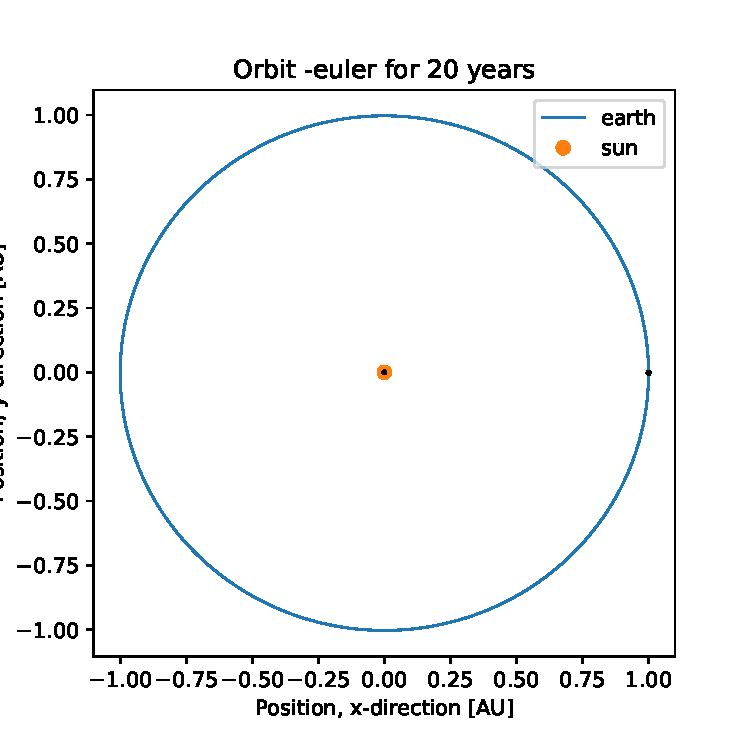
\includegraphics[width=1.1\linewidth]{../results/plots/plotof-earthsun-euler.pdf}\caption{This is a plot of the earth's orbit for 100 years using Euler's method, with 1000 timesteps per year, to simulate the motion.}\label{fig:earth-sun-euler}
\end{figure}		
	
\begin{figure}[H]
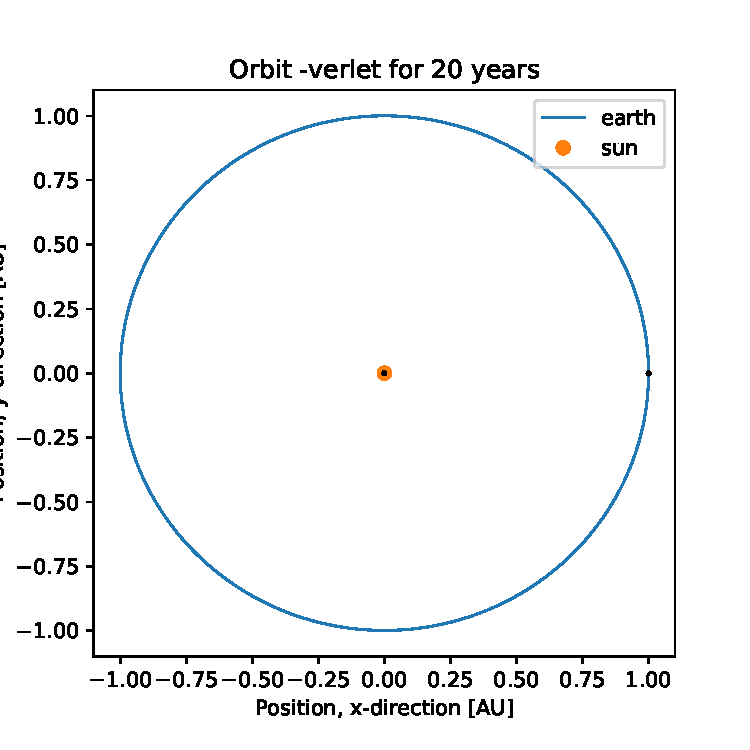
\includegraphics[width=1.1\linewidth]{../results/plots/plotof-earthsun-verlet.pdf}\caption{This is a plot of the earth's orbit for 100 years using the velocity Verlet method, with 1000 timesteps per year, to simulate the motion.}\label{fig:earth-sun-verlet}
\end{figure}	

	- Check that angular moment is conserved
\begin{figure}[H]
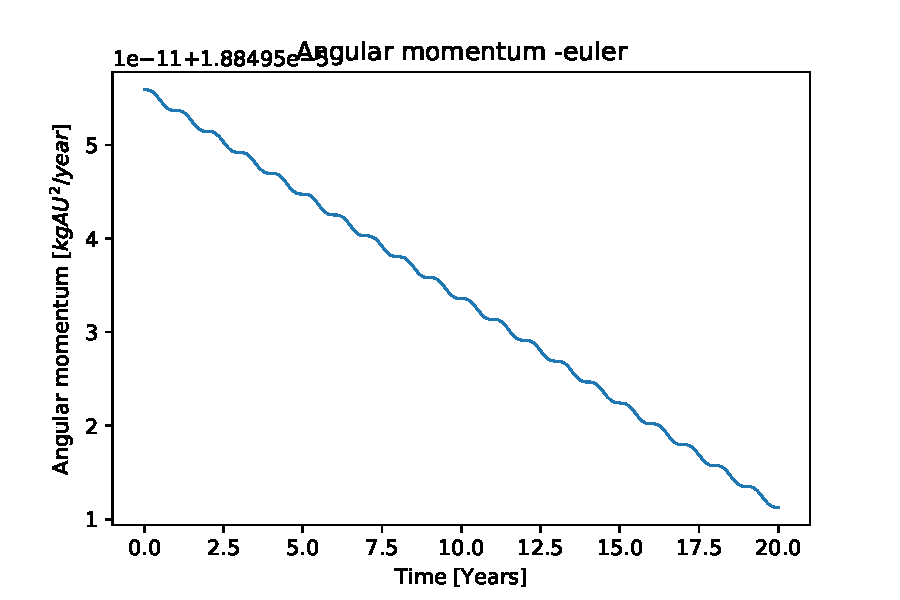
\includegraphics[width=1.1\linewidth]{../results/plots/angularmomentum-euler.pdf}\caption{This is a plot of the angular momentum of the sun-earth system for 100 years using Euler's method, with 1000 timesteps per year.}\label{fig:angluarmomentum-euler}
\end{figure}	

\begin{figure}[H]
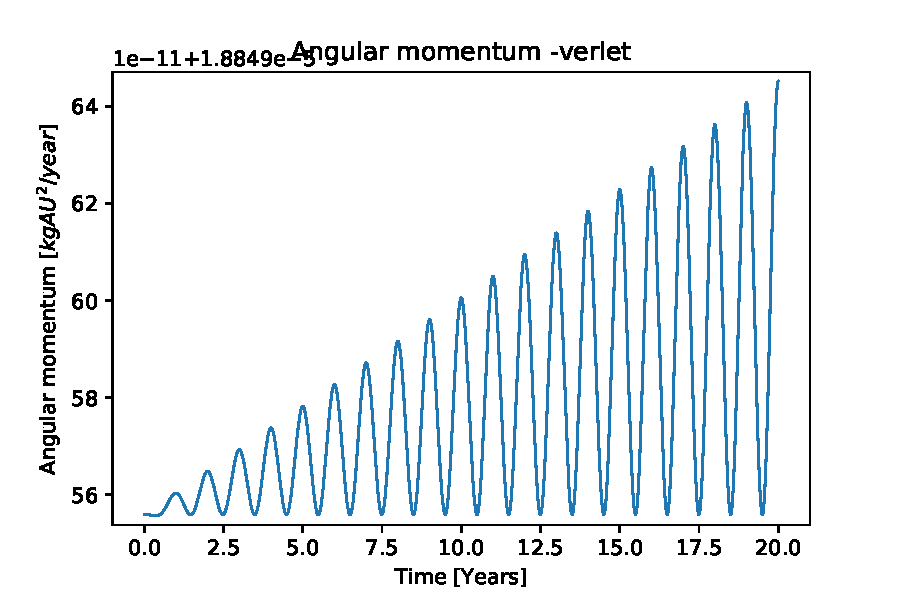
\includegraphics[width=1.1\linewidth]{../results/plots/angularmomentum-verlet.pdf}\caption{This is a plot of the angular momentum of the sun-earth system for 100 years using the velocity Verlet method, with 1000 timesteps per year.}\label{fig:angularmomentum-verlet}
\end{figure}	
	- Check (for the circular orbit) that the energy is conserved (plot - both kin and pot separated and together?)

NEED SOME NUMBERS HERE:

\begin{table}[H]\caption{This is a table that list how the energy oscillates in the two different method (plot in appendix).}\label{tab:energy_oscillations}
\begin{tabular}{ccc}
 & Euler's Method & Velocity Verlet Method\\ \hline
Kinetic energy oscillation & & \\
Potential energy oscillation & & \\
Total energy oscillation & & \\
\end{tabular}
\end{table}

Put these in the appendix?

\begin{figure}[H]
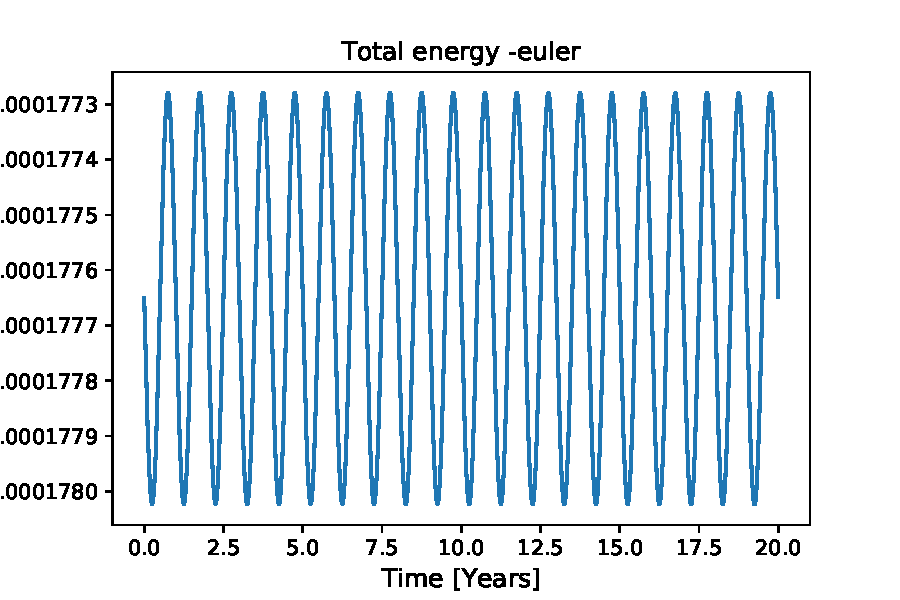
\includegraphics[width=1.1\linewidth]{../results/plots/totalenergy-euler.pdf}\caption{This is a plot of the total energy of the sun-earth system for 100 years using Euler's method, with 1000 timesteps per year.}\label{fig:totalenergy-euler}
\end{figure}	

\begin{figure}[H]
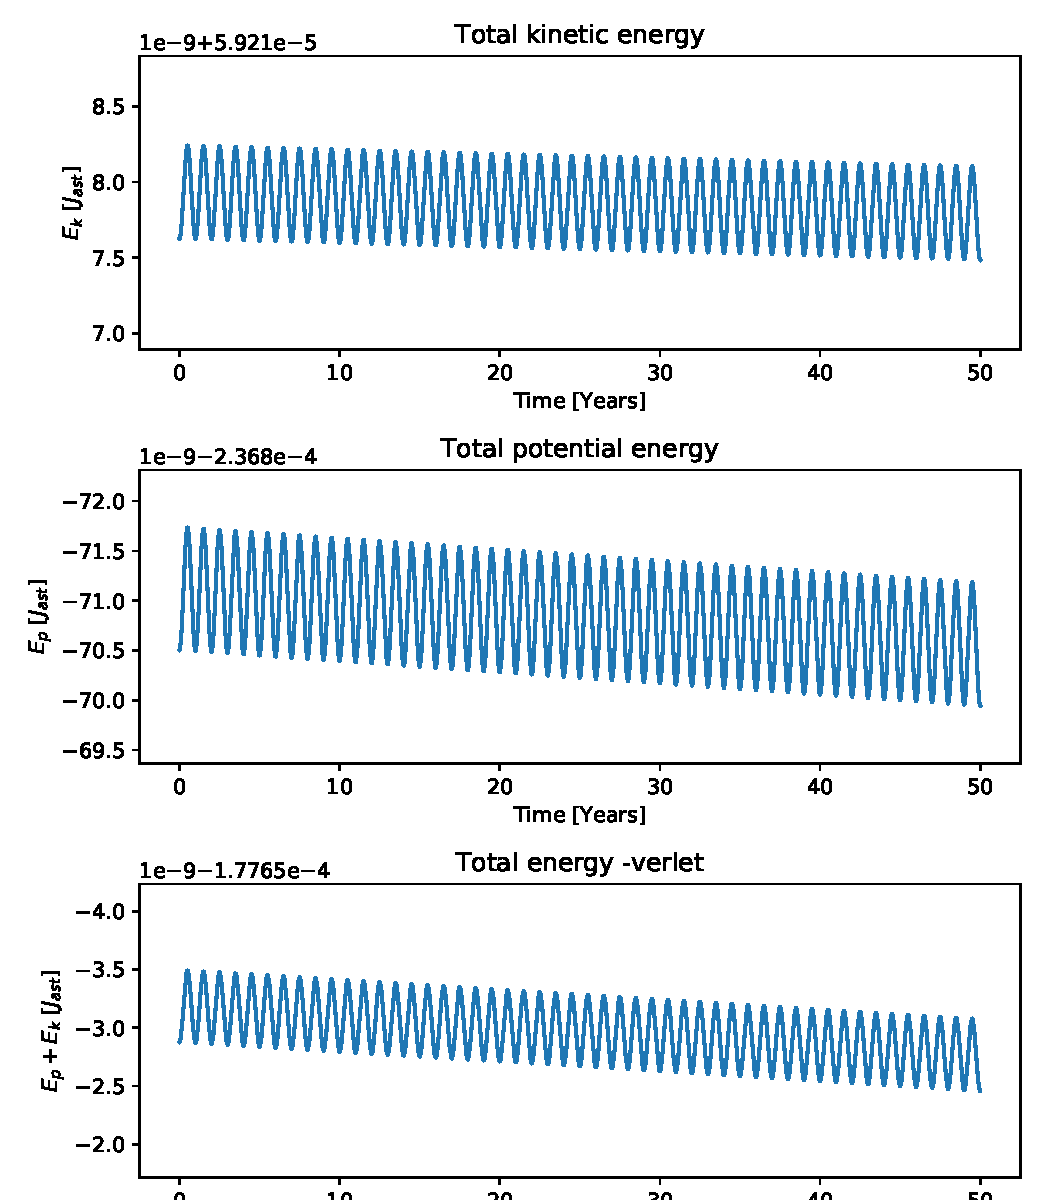
\includegraphics[width=1.1\linewidth]{../results/plots/totalenergy-verlet.pdf}\caption{This is a plot of the total energy of the sun-earth system for 100 years using the velocity Verlet method, with 1000 timesteps per year.}\label{fig:totalenergy-verlet}
\end{figure}

	- Find escape velocity (plot)
	 	- Compare exact and numerical results
	 	
\begin{figure}[H]
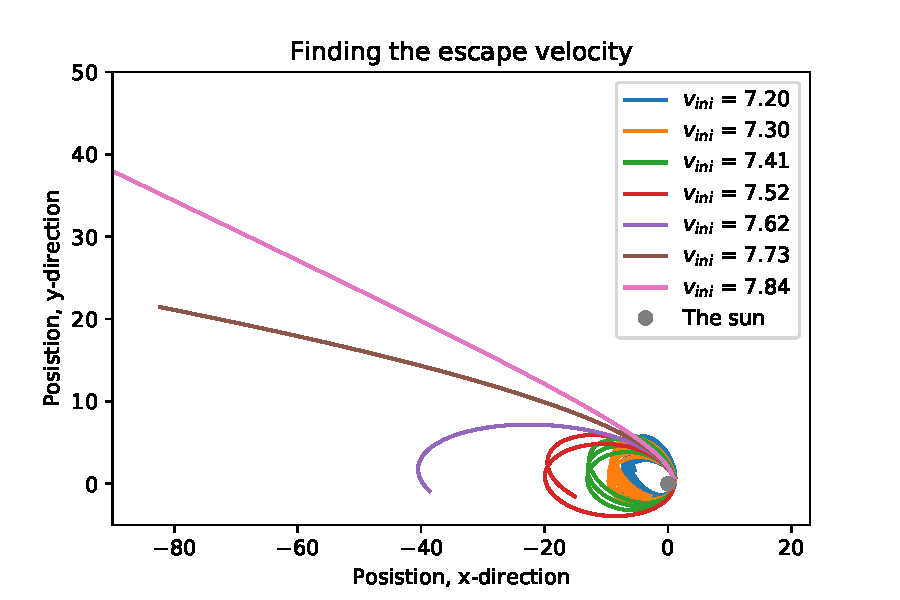
\includegraphics[width=1.1\linewidth]{../results/plots/escape_velocity.pdf}\caption{This is a plot of the sun-earth system for different initial velocities. The plot shows the necesary inital velocity to escape the sun.}\label{fig:escape_velocity}
\end{figure}

\begin{figure}[H]
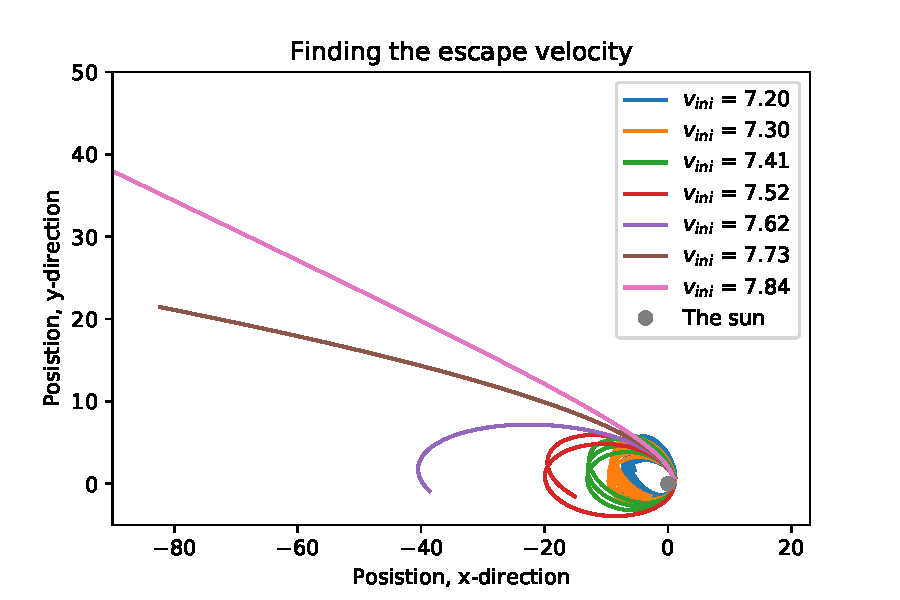
\includegraphics[width=1.1\linewidth]{../results/plots/escape_velocity.pdf}\caption{This is a plot of the sun-earth system for different initial velocities. The plot shows initial velocities near the exact escapevelocity, $\sqrt{2}2\pi$.}\label{fig:escape_velocity_near_exact}
\end{figure}

	- Find exact escape velocity (theory?)

Exact escape velocity:
$$ E_p + E_k = 0 + 0 \implies \frac{g M_E M_S}{r^2} =\frac{1}{2}M_Ev^2$$
$$ v^2 = \frac{4 \pi^2 M_E}{M_E  1^2} AU^2 \implies v = \sqrt{2}2\pi$$

	- Changing beta (plot)
		- Comment result + What happens when beta -> 3 ? (last part in discussion?

\begin{figure}[H]
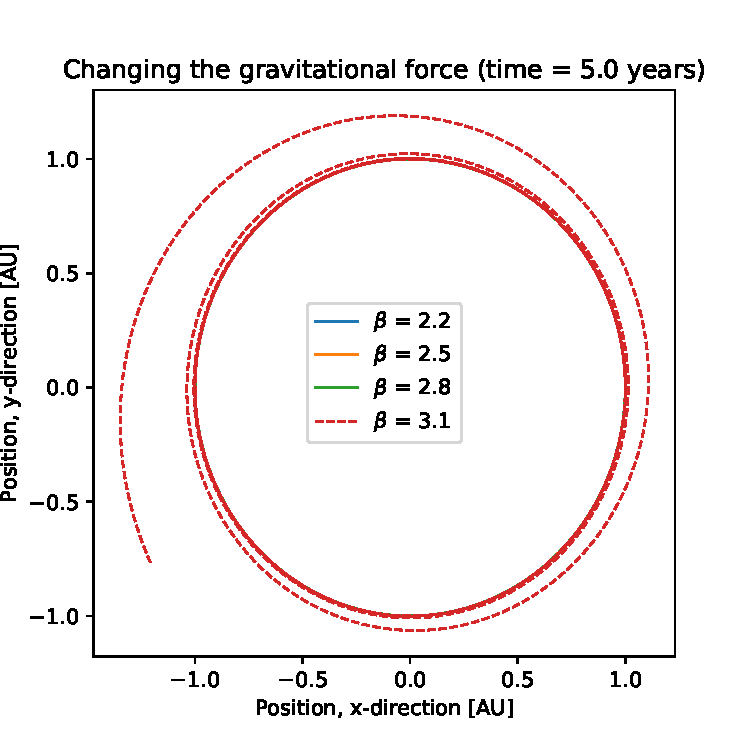
\includegraphics[width=1.1\linewidth]{../results/plots/diffenrent_gravitation.pdf}\caption{This is a plot of the sun-earth system for different gravitational forces. The gravitational force is given by $ F = \frac{-GM_EM_S}{r^\beta}$ and in the plot $\beta$ is changed from it's normal value $\beta = 2$ to $\beta = 3.1$.}\label{fig:different_gravitation}
\end{figure}

	- How much does Jupiter alter Earth's orbit?
	- Position of Jupiter and Earth (plot)	
	
	

	Ok - if initial values are correct.
	
	- Plot Earth's motion for increased mass of Jupiter (3 masses)

	same.	
	
	- Find center off mass - use as origin

	Found and incorporated.	
	
	- Give sun initial velocity so momentum is zero (origin is fixed)

	How? What momentum? velocity?	
	
	- Compare with 3e)
	- Extend to all planets (plot)
	
\begin{figure}[H]
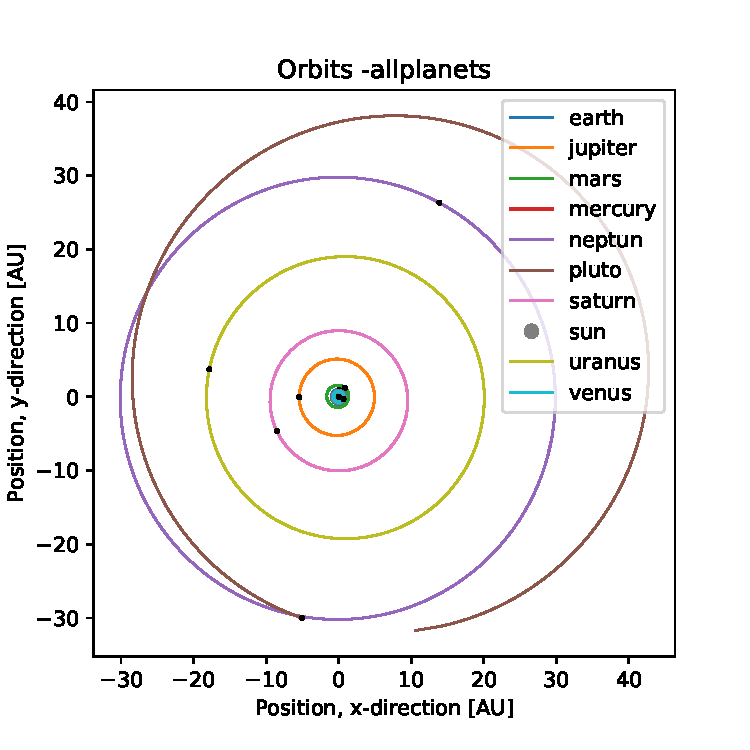
\includegraphics[width=1\linewidth]{../results/plots/plotof-earthjupiter-allplanets.pdf}\caption{This is a plot of the Solar System after 200 years of motion.}\label{fig:solarsystem_allplanets}
\end{figure}


\begin{figure}[H]
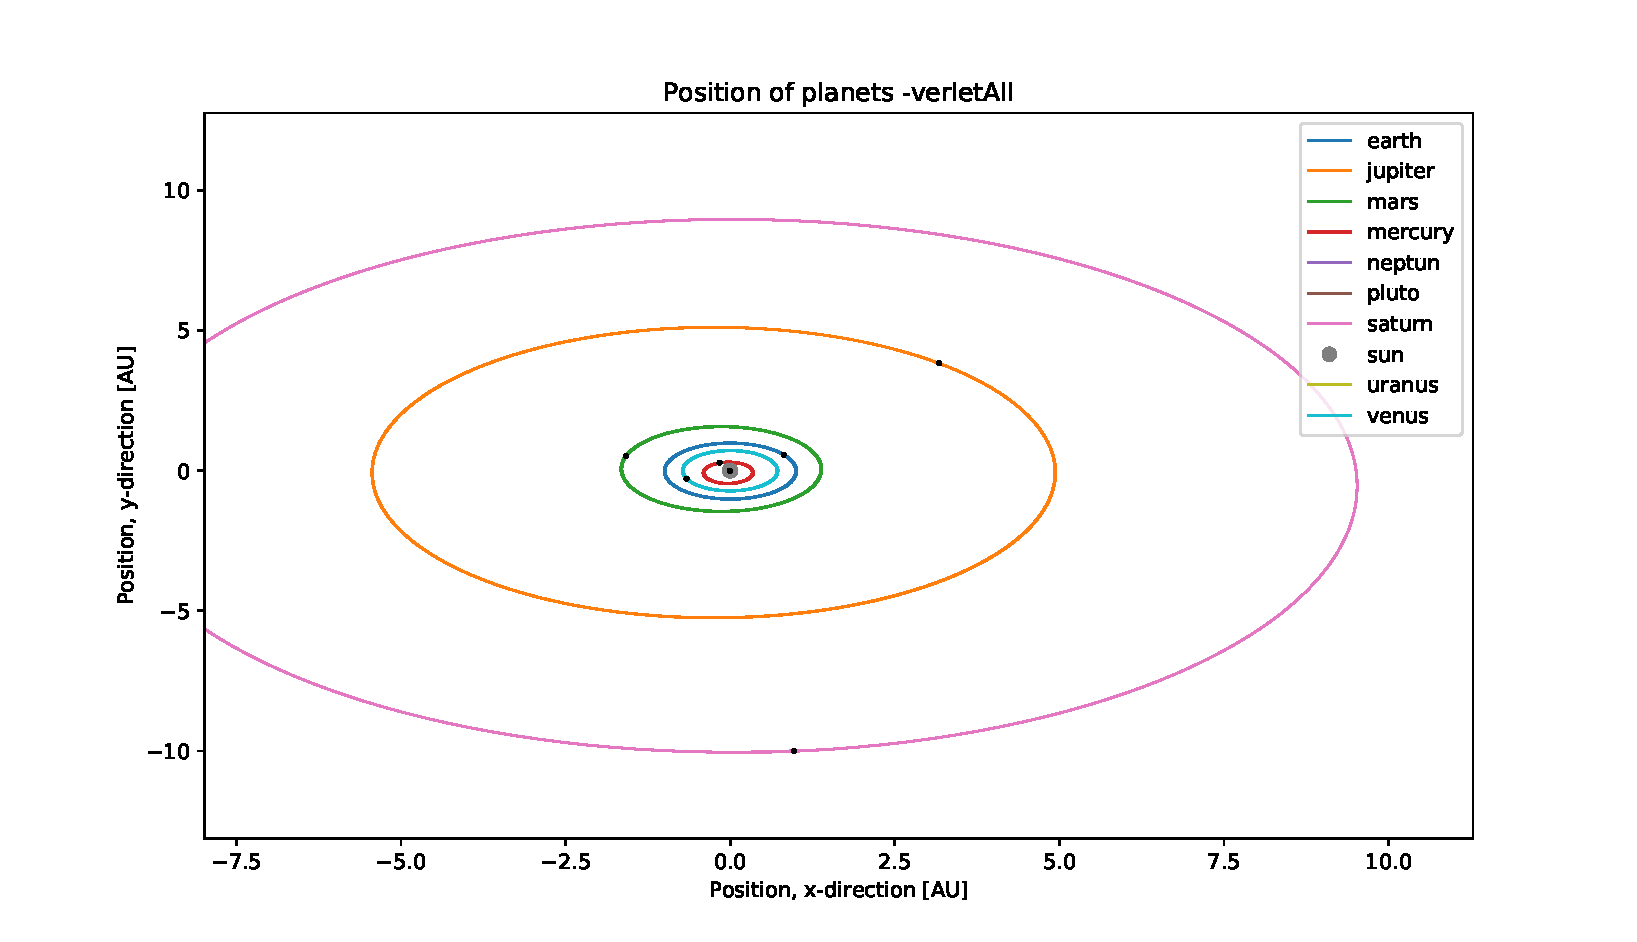
\includegraphics[width=1\linewidth]{../results/plots/innerplanets-verletAll.pdf}\caption{This is a plot of planets closest to the sun in the Solar System after 30 years of motion.}\label{fig:solarsystem_innerplanets}
\end{figure}
	
	- Find perihelion for both relativistic and non-relativistic (table)
	
\begin{table}\caption{This is a table with the Perihelion information about Mercury after one century, 100 years.}\label{tab:Perihelion}
\begin{tabular}{ccc}
 & Newtonian & Relativistic\\ \hline
Position [AU]: & ( , ) & ( , )\\
Angle [arcseconds]: & & \\
\end{tabular}
\end{table}

	- Relativistic - should be a few magnitudes smaller.	

	-  Can the observed perihelion
precession of Mercury be explained by the general theory of relativity?
